% Options for packages loaded elsewhere
\PassOptionsToPackage{unicode}{hyperref}
\PassOptionsToPackage{hyphens}{url}
%
\documentclass[
]{article}
\usepackage{lmodern}
\usepackage{amssymb,amsmath}
\usepackage{ifxetex,ifluatex}
\ifnum 0\ifxetex 1\fi\ifluatex 1\fi=0 % if pdftex
  \usepackage[T1]{fontenc}
  \usepackage[utf8]{inputenc}
  \usepackage{textcomp} % provide euro and other symbols
\else % if luatex or xetex
  \usepackage{unicode-math}
  \defaultfontfeatures{Scale=MatchLowercase}
  \defaultfontfeatures[\rmfamily]{Ligatures=TeX,Scale=1}
\fi
% Use upquote if available, for straight quotes in verbatim environments
\IfFileExists{upquote.sty}{\usepackage{upquote}}{}
\IfFileExists{microtype.sty}{% use microtype if available
  \usepackage[]{microtype}
  \UseMicrotypeSet[protrusion]{basicmath} % disable protrusion for tt fonts
}{}
\makeatletter
\@ifundefined{KOMAClassName}{% if non-KOMA class
  \IfFileExists{parskip.sty}{%
    \usepackage{parskip}
  }{% else
    \setlength{\parindent}{0pt}
    \setlength{\parskip}{6pt plus 2pt minus 1pt}}
}{% if KOMA class
  \KOMAoptions{parskip=half}}
\makeatother
\usepackage{xcolor}
\IfFileExists{xurl.sty}{\usepackage{xurl}}{} % add URL line breaks if available
\IfFileExists{bookmark.sty}{\usepackage{bookmark}}{\usepackage{hyperref}}
\hypersetup{
  pdftitle={Calibrating a 3-state cancer model},
  pdfauthor={The DARTH workgroup},
  hidelinks,
  pdfcreator={LaTeX via pandoc}}
\urlstyle{same} % disable monospaced font for URLs
\usepackage[margin=1in]{geometry}
\usepackage{color}
\usepackage{fancyvrb}
\newcommand{\VerbBar}{|}
\newcommand{\VERB}{\Verb[commandchars=\\\{\}]}
\DefineVerbatimEnvironment{Highlighting}{Verbatim}{commandchars=\\\{\}}
% Add ',fontsize=\small' for more characters per line
\usepackage{framed}
\definecolor{shadecolor}{RGB}{248,248,248}
\newenvironment{Shaded}{\begin{snugshade}}{\end{snugshade}}
\newcommand{\AlertTok}[1]{\textcolor[rgb]{0.94,0.16,0.16}{#1}}
\newcommand{\AnnotationTok}[1]{\textcolor[rgb]{0.56,0.35,0.01}{\textbf{\textit{#1}}}}
\newcommand{\AttributeTok}[1]{\textcolor[rgb]{0.77,0.63,0.00}{#1}}
\newcommand{\BaseNTok}[1]{\textcolor[rgb]{0.00,0.00,0.81}{#1}}
\newcommand{\BuiltInTok}[1]{#1}
\newcommand{\CharTok}[1]{\textcolor[rgb]{0.31,0.60,0.02}{#1}}
\newcommand{\CommentTok}[1]{\textcolor[rgb]{0.56,0.35,0.01}{\textit{#1}}}
\newcommand{\CommentVarTok}[1]{\textcolor[rgb]{0.56,0.35,0.01}{\textbf{\textit{#1}}}}
\newcommand{\ConstantTok}[1]{\textcolor[rgb]{0.00,0.00,0.00}{#1}}
\newcommand{\ControlFlowTok}[1]{\textcolor[rgb]{0.13,0.29,0.53}{\textbf{#1}}}
\newcommand{\DataTypeTok}[1]{\textcolor[rgb]{0.13,0.29,0.53}{#1}}
\newcommand{\DecValTok}[1]{\textcolor[rgb]{0.00,0.00,0.81}{#1}}
\newcommand{\DocumentationTok}[1]{\textcolor[rgb]{0.56,0.35,0.01}{\textbf{\textit{#1}}}}
\newcommand{\ErrorTok}[1]{\textcolor[rgb]{0.64,0.00,0.00}{\textbf{#1}}}
\newcommand{\ExtensionTok}[1]{#1}
\newcommand{\FloatTok}[1]{\textcolor[rgb]{0.00,0.00,0.81}{#1}}
\newcommand{\FunctionTok}[1]{\textcolor[rgb]{0.00,0.00,0.00}{#1}}
\newcommand{\ImportTok}[1]{#1}
\newcommand{\InformationTok}[1]{\textcolor[rgb]{0.56,0.35,0.01}{\textbf{\textit{#1}}}}
\newcommand{\KeywordTok}[1]{\textcolor[rgb]{0.13,0.29,0.53}{\textbf{#1}}}
\newcommand{\NormalTok}[1]{#1}
\newcommand{\OperatorTok}[1]{\textcolor[rgb]{0.81,0.36,0.00}{\textbf{#1}}}
\newcommand{\OtherTok}[1]{\textcolor[rgb]{0.56,0.35,0.01}{#1}}
\newcommand{\PreprocessorTok}[1]{\textcolor[rgb]{0.56,0.35,0.01}{\textit{#1}}}
\newcommand{\RegionMarkerTok}[1]{#1}
\newcommand{\SpecialCharTok}[1]{\textcolor[rgb]{0.00,0.00,0.00}{#1}}
\newcommand{\SpecialStringTok}[1]{\textcolor[rgb]{0.31,0.60,0.02}{#1}}
\newcommand{\StringTok}[1]{\textcolor[rgb]{0.31,0.60,0.02}{#1}}
\newcommand{\VariableTok}[1]{\textcolor[rgb]{0.00,0.00,0.00}{#1}}
\newcommand{\VerbatimStringTok}[1]{\textcolor[rgb]{0.31,0.60,0.02}{#1}}
\newcommand{\WarningTok}[1]{\textcolor[rgb]{0.56,0.35,0.01}{\textbf{\textit{#1}}}}
\usepackage{graphicx,grffile}
\makeatletter
\def\maxwidth{\ifdim\Gin@nat@width>\linewidth\linewidth\else\Gin@nat@width\fi}
\def\maxheight{\ifdim\Gin@nat@height>\textheight\textheight\else\Gin@nat@height\fi}
\makeatother
% Scale images if necessary, so that they will not overflow the page
% margins by default, and it is still possible to overwrite the defaults
% using explicit options in \includegraphics[width, height, ...]{}
\setkeys{Gin}{width=\maxwidth,height=\maxheight,keepaspectratio}
% Set default figure placement to htbp
\makeatletter
\def\fps@figure{htbp}
\makeatother
\setlength{\emergencystretch}{3em} % prevent overfull lines
\providecommand{\tightlist}{%
  \setlength{\itemsep}{0pt}\setlength{\parskip}{0pt}}
\setcounter{secnumdepth}{-\maxdimen} % remove section numbering

\title{Calibrating a 3-state cancer model}
\usepackage{etoolbox}
\makeatletter
\providecommand{\subtitle}[1]{% add subtitle to \maketitle
  \apptocmd{\@title}{\par {\large #1 \par}}{}{}
}
\makeatother
\subtitle{Directed search using Nelder-mead}
\author{The DARTH workgroup}
\date{}

\begin{document}
\maketitle

Developed by the Decision Analysis in R for Technologies in Health
(DARTH) workgroup:

Fernando Alarid-Escudero, PhD (1)

Eva A. Enns, MS, PhD (2)

M.G. Myriam Hunink, MD, PhD (3,4)

Hawre J. Jalal, MD, PhD (5)

Eline M. Krijkamp, MSc (3)

Petros Pechlivanoglou, PhD (6)

Alan Yang, MSc (7)

In collaboration of:

\begin{enumerate}
\def\labelenumi{\arabic{enumi}.}
\tightlist
\item
  Division of Public Administration, Center for Research and Teaching in
  Economics (CIDE), Aguascalientes, Mexico
\item
  University of Minnesota School of Public Health, Minneapolis, MN, USA
\item
  Erasmus MC, Rotterdam, The Netherlands
\item
  Harvard T.H. Chan School of Public Health, Boston, USA
\item
  University of Pittsburgh Graduate School of Public Health, Pittsburgh,
  PA, USA
\item
  The Hospital for Sick Children, Toronto and University of Toronto,
  Toronto ON, Canada
\item
  The Hospital for Sick Children, Toronto ON, Canada
\end{enumerate}

Please cite our publications when using this code:

\begin{itemize}
\item
  Alarid-Escudero F, Maclehose RF, Peralta Y, Kuntz KM, Enns EA.
  Non-identifiability in model calibration and implications for medical
  decision making. Med Decis Making. 2018; 38(7):810-821.
  \url{https://pubmed.ncbi.nlm.nih.gov/30248276/}
\item
  Jalal H, Pechlivanoglou P, Krijkamp E, Alarid-Escudero F, Enns E,
  Hunink MG. An Overview of R in Health Decision Sciences. Med Decis
  Making. 2017; 37(3): 735-746.
  \url{https://journals.sagepub.com/doi/abs/10.1177/0272989X16686559}
\end{itemize}

A walkthrough of the code could be found in the following link: -
\url{https://darth-git.github.io/calibSMDM2018-materials/}

Copyright 2017, THE HOSPITAL FOR SICK CHILDREN AND THE COLLABORATING
INSTITUTIONS. All rights reserved in Canada, the United States and
worldwide. Copyright, trademarks, trade names and any and all associated
intellectual property are exclusively owned by THE HOSPITAL FOR Sick
CHILDREN and the collaborating institutions. These materials may be
used, reproduced, modified, distributed and adapted with proper
attribution.

\newpage

\begin{Shaded}
\begin{Highlighting}[]
\KeywordTok{rm}\NormalTok{(}\DataTypeTok{list =} \KeywordTok{ls}\NormalTok{())      }\CommentTok{# clear memory (removes all the variables from the workspace)}
\end{Highlighting}
\end{Shaded}

\hypertarget{calibration-specifications}{%
\section{00 Calibration
Specifications}\label{calibration-specifications}}

Model: 3-State Cancer Relative Survival (CRS) Markov Model

Inputs to be calibrated: p\_Mets, p\_DieMets

Targets: Surv

Calibration method: Directed search using Nelder-mead

Goodness-of-fit measure: Sum of Log-Likelihood

\hypertarget{load-packages}{%
\section{01 Load packages}\label{load-packages}}

\begin{Shaded}
\begin{Highlighting}[]
\ControlFlowTok{if}\NormalTok{ (}\OperatorTok{!}\KeywordTok{require}\NormalTok{(}\StringTok{'pacman'}\NormalTok{)) \{}
  \KeywordTok{install.packages}\NormalTok{(}\StringTok{'pacman'}\NormalTok{)}
\NormalTok{\}}
\KeywordTok{library}\NormalTok{(pacman) }\CommentTok{# use this package to conveniently install other packages}
\CommentTok{# load (install if required) packages from CRAN}
\KeywordTok{p_load}\NormalTok{(}\StringTok{"lhs"}\NormalTok{, }\StringTok{"plotrix"}\NormalTok{, }\StringTok{"psych"}\NormalTok{, }\StringTok{"pacman"}\NormalTok{)  }
\end{Highlighting}
\end{Shaded}

\hypertarget{load-target-data}{%
\section{02 Load target data}\label{load-target-data}}

\begin{Shaded}
\begin{Highlighting}[]
\KeywordTok{load}\NormalTok{(}\StringTok{"CRS_CalibTargets.RData"}\NormalTok{)}
\NormalTok{lst_targets <-}\StringTok{ }\NormalTok{CRS_targets}

\CommentTok{# Plot the targets}

\CommentTok{# TARGET 1: Survival ("Surv")}
\NormalTok{plotrix}\OperatorTok{::}\KeywordTok{plotCI}\NormalTok{(}\DataTypeTok{x =}\NormalTok{ lst_targets}\OperatorTok{$}\NormalTok{Surv}\OperatorTok{$}\NormalTok{time, }\DataTypeTok{y =}\NormalTok{ lst_targets}\OperatorTok{$}\NormalTok{Surv}\OperatorTok{$}\NormalTok{value, }
                \DataTypeTok{ui =}\NormalTok{ lst_targets}\OperatorTok{$}\NormalTok{Surv}\OperatorTok{$}\NormalTok{ub,}
                \DataTypeTok{li =}\NormalTok{ lst_targets}\OperatorTok{$}\NormalTok{Surv}\OperatorTok{$}\NormalTok{lb,}
                \DataTypeTok{ylim =} \KeywordTok{c}\NormalTok{(}\DecValTok{0}\NormalTok{, }\DecValTok{1}\NormalTok{), }
                \DataTypeTok{xlab =} \StringTok{"Time"}\NormalTok{, }\DataTypeTok{ylab =} \StringTok{"Pr Survive"}\NormalTok{)}
\end{Highlighting}
\end{Shaded}

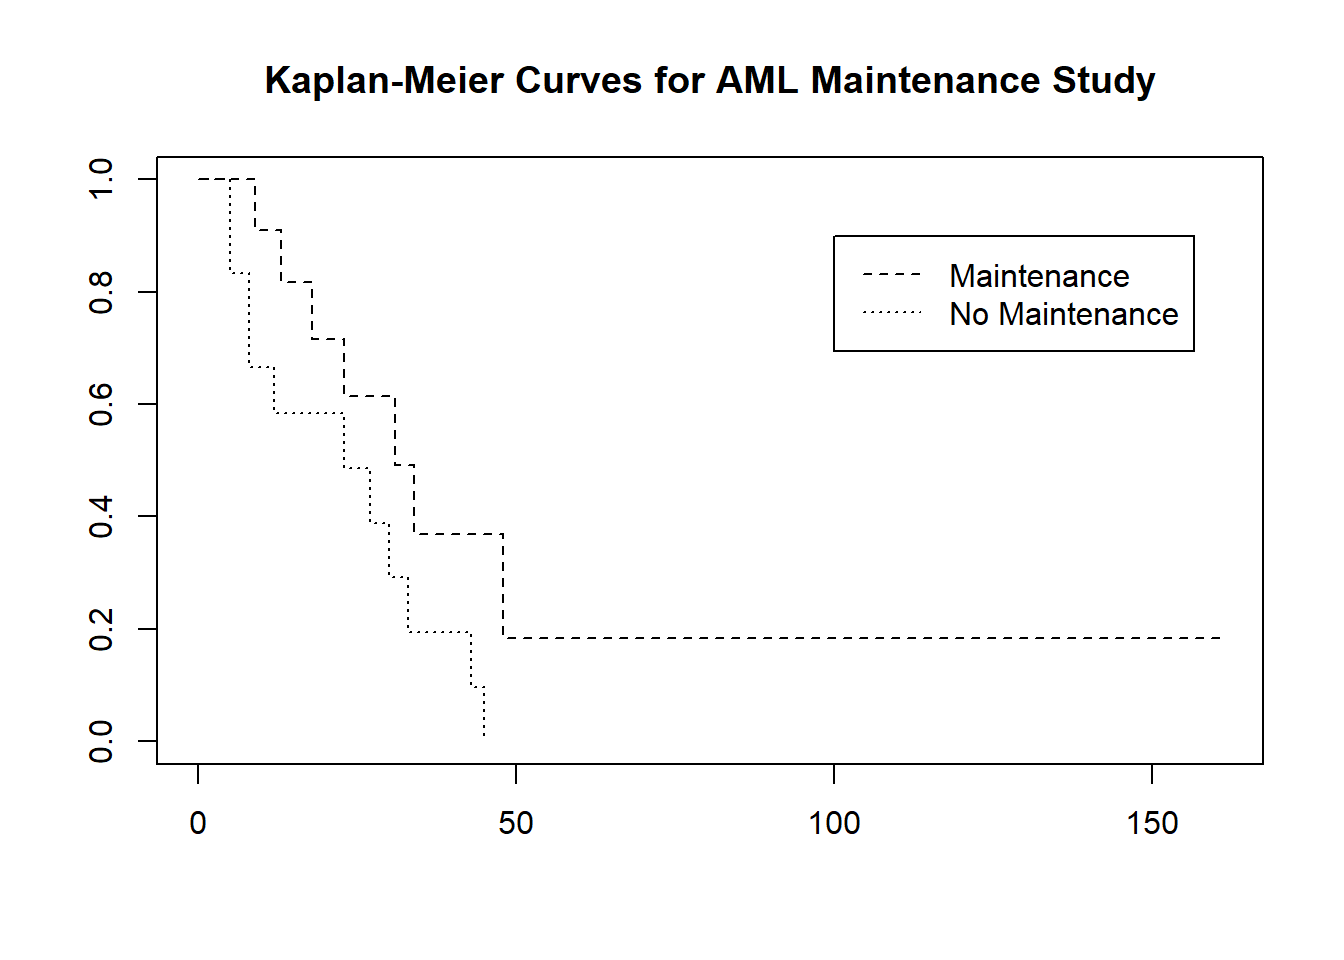
\includegraphics{CRS_Calib_NelderMead_files/figure-latex/unnamed-chunk-3-1.pdf}

\begin{Shaded}
\begin{Highlighting}[]
\CommentTok{# TARGET 2: (if you had more...)}
\CommentTok{# plotrix::plotCI(x = lst_targets$Target2$time, y = lst_targets$Target2$value, }
\CommentTok{#                 ui = lst_targets$Target2$ub,}
\CommentTok{#                 li = lst_targets$Target2$lb,}
\CommentTok{#                 ylim = c(0, 1), }
\CommentTok{#                 xlab = "Time", ylab = "Target 2")}
\end{Highlighting}
\end{Shaded}

\hypertarget{load-model-as-a-function}{%
\section{03 Load model as a function}\label{load-model-as-a-function}}

\begin{Shaded}
\begin{Highlighting}[]
\CommentTok{# - inputs are parameters to be estimated through calibration}
\CommentTok{# - outputs correspond to the target data}

\KeywordTok{source}\NormalTok{(}\StringTok{"CRS_MarkovModel_Function.R"}\NormalTok{) }\CommentTok{# creates the function run_crs_markov()}

\CommentTok{# Check that it works}
\NormalTok{v_params_test <-}\StringTok{ }\KeywordTok{c}\NormalTok{(}\DataTypeTok{p_Mets =} \FloatTok{0.10}\NormalTok{, }\DataTypeTok{p_DieMets =} \FloatTok{0.05}\NormalTok{)}
\KeywordTok{run_crs_markov}\NormalTok{(v_params_test) }\CommentTok{# It works!}
\end{Highlighting}
\end{Shaded}

\begin{verbatim}
## $Surv
##          2          3          4          5          6          7          8 
## 0.99500000 0.98575000 0.97291250 0.95707188 0.93874278 0.91837769 0.89637365 
##          9         10         11         12         13         14         15 
## 0.87307833 0.84879544 0.82378959 0.79829064 0.77249758 0.74658203 0.72069133 
##         16         17         18         19         20         21         22 
## 0.69495132 0.66946885 0.64433400 0.61962203 0.59539519 0.57170426 0.54859000 
##         23         24         25         26         27         28         29 
## 0.52608435 0.50421161 0.48298935 0.46242937 0.44253844 0.42331901 0.40476980 
##         30         31         32         33         34         35         36 
## 0.38688637 0.36966161 0.35308613 0.33714867 0.32183639 0.30713521 0.29303003 
##         37         38         39         40         41         42         43 
## 0.27950495 0.26654348 0.25412871 0.24224343 0.23087030 0.21999193 0.20959096 
##         44         45         46         47         48         49         50 
## 0.19965017 0.19015255 0.18108132 0.17242001 0.16415250 0.15626300 0.14873618 
##         51         52         53         54         55         56         57 
## 0.14155706 0.13471112 0.12818429 0.12196293 0.11603386 0.11038433 0.10500206 
##         58         59         60 
## 0.09987521 0.09499237 0.09034259
\end{verbatim}

\hypertarget{specify-calibration-parameters}{%
\section{04 Specify calibration
parameters}\label{specify-calibration-parameters}}

\begin{Shaded}
\begin{Highlighting}[]
\CommentTok{# Specify seed (for reproducible sequence of random numbers)}
\KeywordTok{set.seed}\NormalTok{(}\DecValTok{072218}\NormalTok{)}

\CommentTok{# number of initial starting points}
\NormalTok{n_init <-}\StringTok{ }\DecValTok{100}

\CommentTok{# names and number of input parameters to be calibrated}
\NormalTok{v_param_names <-}\StringTok{ }\KeywordTok{c}\NormalTok{(}\StringTok{"p_Mets"}\NormalTok{,}\StringTok{"p_DieMets"}\NormalTok{)}
\NormalTok{n_param <-}\StringTok{ }\KeywordTok{length}\NormalTok{(v_param_names)}

\CommentTok{# range on input search space}
\NormalTok{lb <-}\StringTok{ }\KeywordTok{c}\NormalTok{(}\DataTypeTok{p_Mets =} \FloatTok{0.04}\NormalTok{, }\DataTypeTok{p_DieMets =} \FloatTok{0.04}\NormalTok{) }\CommentTok{# lower bound}
\NormalTok{ub <-}\StringTok{ }\KeywordTok{c}\NormalTok{(}\DataTypeTok{p_Mets =} \FloatTok{0.16}\NormalTok{, }\DataTypeTok{p_DieMets =} \FloatTok{0.16}\NormalTok{) }\CommentTok{# upper bound}

\CommentTok{# number of calibration targets}
\NormalTok{v_target_names <-}\StringTok{ }\KeywordTok{c}\NormalTok{(}\StringTok{"Surv"}\NormalTok{)}
\NormalTok{n_target <-}\StringTok{ }\KeywordTok{length}\NormalTok{(v_target_names)}
\end{Highlighting}
\end{Shaded}

\hypertarget{calibration-functions}{%
\section{05 Calibration functions}\label{calibration-functions}}

\begin{Shaded}
\begin{Highlighting}[]
\CommentTok{# Write goodness-of-fit function to pass to Nelder-Mead algorithm}
\NormalTok{f_gof <-}\StringTok{ }\ControlFlowTok{function}\NormalTok{(v_params)\{}
  
  \CommentTok{# Run model for parametr set "v_params"}
\NormalTok{  model_res <-}\StringTok{ }\KeywordTok{run_crs_markov}\NormalTok{(v_params)}
  
  \CommentTok{# Calculate goodness-of-fit of model outputs to targets}
\NormalTok{  v_GOF <-}\StringTok{ }\KeywordTok{numeric}\NormalTok{(n_target)}
  \CommentTok{# TARGET 1: Survival ("Surv")}
  \CommentTok{# log likelihood  }
\NormalTok{  v_GOF[}\DecValTok{1}\NormalTok{] <-}\StringTok{ }\KeywordTok{sum}\NormalTok{(}\KeywordTok{dnorm}\NormalTok{(}\DataTypeTok{x =}\NormalTok{ lst_targets}\OperatorTok{$}\NormalTok{Surv}\OperatorTok{$}\NormalTok{value,}
                        \DataTypeTok{mean =}\NormalTok{ model_res}\OperatorTok{$}\NormalTok{Surv,}
                        \DataTypeTok{sd =}\NormalTok{ lst_targets}\OperatorTok{$}\NormalTok{Surv}\OperatorTok{$}\NormalTok{se,}
                        \DataTypeTok{log =}\NormalTok{ T))}
  
  \CommentTok{# TARGET 2: (if you had more...)}
  \CommentTok{# log likelihood}
  \CommentTok{# v_GOF[2] <- sum(dnorm(x = lst_targets$Target2$value,}
  \CommentTok{#                        mean = model_res$Target2,}
  \CommentTok{#                        sd = lst_targets$Target2$se,}
  \CommentTok{#                        log = T))}
  
  \CommentTok{# OVERALL}
  \CommentTok{# can give different targets different weights}
\NormalTok{  v_weights <-}\StringTok{ }\KeywordTok{rep}\NormalTok{(}\DecValTok{1}\NormalTok{,n_target)}
  \CommentTok{# weighted sum}
\NormalTok{  GOF_overall <-}\StringTok{ }\KeywordTok{sum}\NormalTok{(v_GOF[}\DecValTok{1}\OperatorTok{:}\NormalTok{n_target] }\OperatorTok{*}\StringTok{ }\NormalTok{v_weights)}
  
  \CommentTok{# return GOF}
  \KeywordTok{return}\NormalTok{(GOF_overall)}
\NormalTok{\}}
\end{Highlighting}
\end{Shaded}

\hypertarget{calibrate}{%
\section{06 Calibrate!}\label{calibrate}}

\begin{Shaded}
\begin{Highlighting}[]
\CommentTok{# record start time of calibration}
\NormalTok{t_init <-}\StringTok{ }\KeywordTok{Sys.time}\NormalTok{()}

\CommentTok{###  Sample multiple random starting values for Nelder-Mead  }\AlertTok{###}
\NormalTok{v_params_init <-}\StringTok{ }\KeywordTok{matrix}\NormalTok{(}\DataTypeTok{nrow=}\NormalTok{n_init, }\DataTypeTok{ncol=}\NormalTok{n_param)}
\ControlFlowTok{for}\NormalTok{ (i }\ControlFlowTok{in} \DecValTok{1}\OperatorTok{:}\NormalTok{n_param)\{}
\NormalTok{  v_params_init[,i] <-}\StringTok{ }\KeywordTok{runif}\NormalTok{(n_init,}\DataTypeTok{min=}\NormalTok{lb[i],}\DataTypeTok{max=}\NormalTok{ub[i])}
\NormalTok{\}}
\KeywordTok{colnames}\NormalTok{(v_params_init) <-}\StringTok{ }\NormalTok{v_param_names}

\CommentTok{###  Run Nelder-Mead for each starting point  }\AlertTok{###}
\NormalTok{m_calib_res <-}\StringTok{ }\KeywordTok{matrix}\NormalTok{(}\DataTypeTok{nrow =}\NormalTok{ n_init, }\DataTypeTok{ncol =}\NormalTok{ n_param}\OperatorTok{+}\DecValTok{1}\NormalTok{)}
\KeywordTok{colnames}\NormalTok{(m_calib_res) <-}\StringTok{ }\KeywordTok{c}\NormalTok{(v_param_names, }\StringTok{"Overall_fit"}\NormalTok{)}
\ControlFlowTok{for}\NormalTok{ (j }\ControlFlowTok{in} \DecValTok{1}\OperatorTok{:}\NormalTok{n_init)\{}
  
  \CommentTok{### use optim() as Nelder-Mead }\AlertTok{###}
\NormalTok{  fit_nm <-}\StringTok{ }\KeywordTok{optim}\NormalTok{(v_params_init[j,], f_gof,}
                 \DataTypeTok{control =} \KeywordTok{list}\NormalTok{(}\DataTypeTok{fnscale =} \DecValTok{-1}\NormalTok{, }\CommentTok{# switches from minimization to maximization}
                                \DataTypeTok{maxit =} \DecValTok{1000}\NormalTok{), }\DataTypeTok{hessian =}\NormalTok{ T)}
\NormalTok{  m_calib_res[j,] <-}\StringTok{ }\KeywordTok{c}\NormalTok{(fit_nm}\OperatorTok{$}\NormalTok{par,fit_nm}\OperatorTok{$}\NormalTok{value)}
  
  \CommentTok{### to use a simulated annealing instead }\AlertTok{###}
  \CommentTok{# fit_sa <- optim(v_params_init[j,], f_gof,}
  \CommentTok{#                method = c("SANN"),  # switches to using simulated annealing}
  \CommentTok{#                control = list(temp = 10, tmax = 10, # algorithm tuning parameters}
  \CommentTok{#                               fnscale = -1, maxit = 1000),}
  \CommentTok{#                hessian = T)}
  \CommentTok{# m_calib_res[j,] = c(fit_sa$par,fit_sa$value)}
  
  \CommentTok{### to use a genetic algorithm instead }\AlertTok{###}
  \CommentTok{# library(DEoptim)}
  \CommentTok{# f_fitness <- function(params)\{}
  \CommentTok{#   names(params) = v_param_names}
  \CommentTok{#   return(-f_gof(params))\}}
  \CommentTok{# fit_ga = DEoptim(f_fitness, lower=lb, upper=ub)}
  \CommentTok{# m_calib_res[j,] = c(fit_ga$optim$bestmem,-1*fit_ga$optim$bestval)}

\NormalTok{  \}}

\CommentTok{# Calculate computation time}
\NormalTok{comp_time <-}\StringTok{ }\KeywordTok{Sys.time}\NormalTok{() }\OperatorTok{-}\StringTok{ }\NormalTok{t_init}
\end{Highlighting}
\end{Shaded}

\hypertarget{exploring-best-fitting-input-sets}{%
\section{07 Exploring best-fitting input
sets}\label{exploring-best-fitting-input-sets}}

\begin{Shaded}
\begin{Highlighting}[]
\CommentTok{# Arrange parameter sets in order of fit}
\NormalTok{m_calib_res <-}\StringTok{ }\NormalTok{m_calib_res[}\KeywordTok{order}\NormalTok{(}\OperatorTok{-}\NormalTok{m_calib_res[,}\StringTok{"Overall_fit"}\NormalTok{]),]}

\CommentTok{# Examine the top 10 best-fitting sets}
\NormalTok{m_calib_res[}\DecValTok{1}\OperatorTok{:}\DecValTok{10}\NormalTok{, ]}
\end{Highlighting}
\end{Shaded}

\begin{verbatim}
##           p_Mets  p_DieMets Overall_fit
##  [1,] 0.04810740 0.12439706    156.0328
##  [2,] 0.04810703 0.12439834    156.0328
##  [3,] 0.12439619 0.04810733    156.0328
##  [4,] 0.04810708 0.12439961    156.0328
##  [5,] 0.04810765 0.12439450    156.0328
##  [6,] 0.04810695 0.12439797    156.0328
##  [7,] 0.04810655 0.12440104    156.0328
##  [8,] 0.04810789 0.12439263    156.0328
##  [9,] 0.12439411 0.04810754    156.0328
## [10,] 0.04810769 0.12439731    156.0328
\end{verbatim}

\begin{Shaded}
\begin{Highlighting}[]
\CommentTok{# Plot the top 10 (top 10%)}
\KeywordTok{plot}\NormalTok{(m_calib_res[}\DecValTok{1}\OperatorTok{:}\DecValTok{10}\NormalTok{,}\DecValTok{1}\NormalTok{],m_calib_res[}\DecValTok{1}\OperatorTok{:}\DecValTok{10}\NormalTok{,}\DecValTok{2}\NormalTok{],}
     \DataTypeTok{xlim=}\KeywordTok{c}\NormalTok{(lb[}\DecValTok{1}\NormalTok{],ub[}\DecValTok{1}\NormalTok{]),}\DataTypeTok{ylim=}\KeywordTok{c}\NormalTok{(lb[}\DecValTok{2}\NormalTok{],ub[}\DecValTok{2}\NormalTok{]),}
     \DataTypeTok{xlab =} \KeywordTok{colnames}\NormalTok{(m_calib_res)[}\DecValTok{1}\NormalTok{],}\DataTypeTok{ylab =} \KeywordTok{colnames}\NormalTok{(m_calib_res)[}\DecValTok{2}\NormalTok{])}
\end{Highlighting}
\end{Shaded}

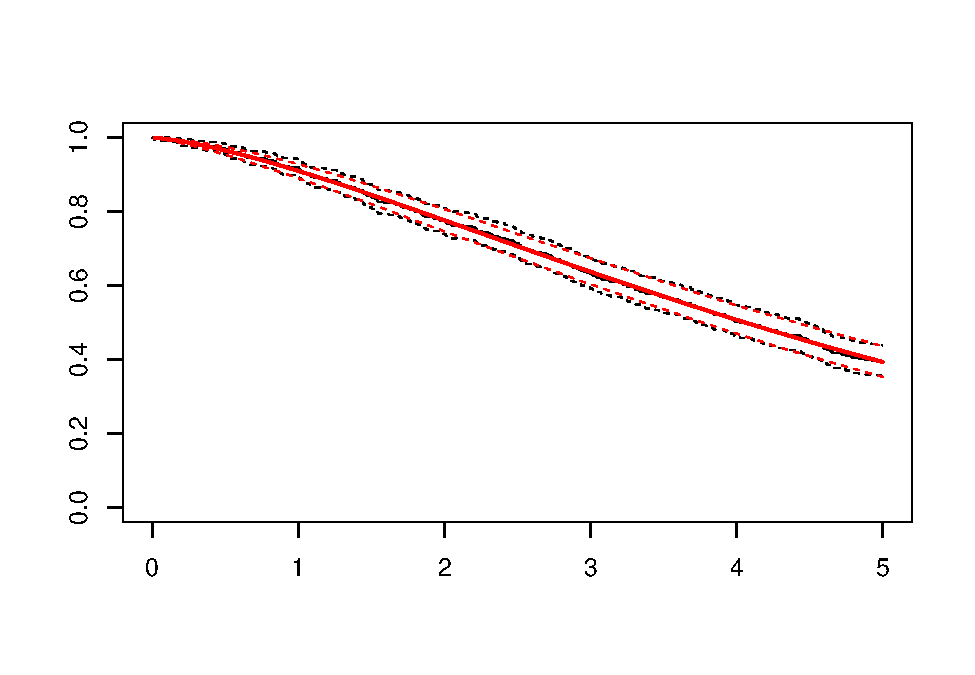
\includegraphics{CRS_Calib_NelderMead_files/figure-latex/unnamed-chunk-8-1.pdf}

\begin{Shaded}
\begin{Highlighting}[]
\CommentTok{# Pairwise comparison of top 10 sets}
\KeywordTok{pairs.panels}\NormalTok{(m_calib_res[}\DecValTok{1}\OperatorTok{:}\DecValTok{10}\NormalTok{,v_param_names])}
\end{Highlighting}
\end{Shaded}

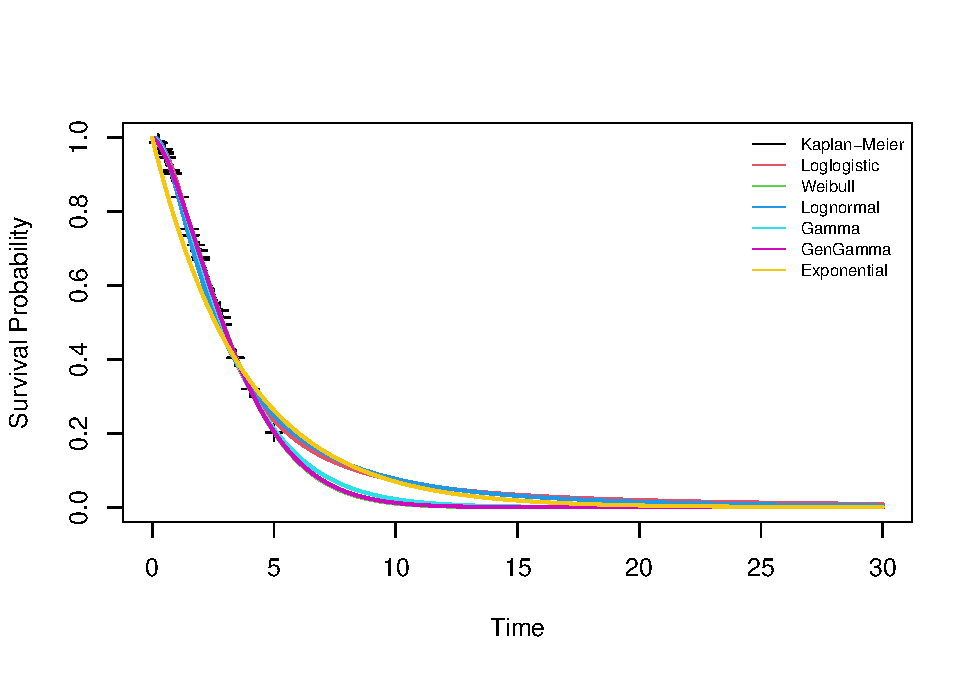
\includegraphics{CRS_Calib_NelderMead_files/figure-latex/unnamed-chunk-8-2.pdf}

\begin{Shaded}
\begin{Highlighting}[]
\CommentTok{### Plot model-predicted output at mean vs targets }\AlertTok{###}
\NormalTok{v_out_best <-}\StringTok{ }\KeywordTok{run_crs_markov}\NormalTok{(m_calib_res[}\DecValTok{1}\NormalTok{,])}

\CommentTok{# TARGET 1: Survival ("Surv")}
\NormalTok{plotrix}\OperatorTok{::}\KeywordTok{plotCI}\NormalTok{(}\DataTypeTok{x =}\NormalTok{ lst_targets}\OperatorTok{$}\NormalTok{Surv}\OperatorTok{$}\NormalTok{time, }\DataTypeTok{y =}\NormalTok{ lst_targets}\OperatorTok{$}\NormalTok{Surv}\OperatorTok{$}\NormalTok{value, }
                \DataTypeTok{ui =}\NormalTok{ lst_targets}\OperatorTok{$}\NormalTok{Surv}\OperatorTok{$}\NormalTok{ub,}
                \DataTypeTok{li =}\NormalTok{ lst_targets}\OperatorTok{$}\NormalTok{Surv}\OperatorTok{$}\NormalTok{lb,}
                \DataTypeTok{ylim =} \KeywordTok{c}\NormalTok{(}\DecValTok{0}\NormalTok{, }\DecValTok{1}\NormalTok{), }
                \DataTypeTok{xlab =} \StringTok{"Time"}\NormalTok{, }\DataTypeTok{ylab =} \StringTok{"Pr Survive"}\NormalTok{)}
\KeywordTok{points}\NormalTok{(}\DataTypeTok{x =}\NormalTok{ lst_targets}\OperatorTok{$}\NormalTok{Surv}\OperatorTok{$}\NormalTok{time, }
       \DataTypeTok{y =}\NormalTok{ v_out_best}\OperatorTok{$}\NormalTok{Surv, }
       \DataTypeTok{pch =} \DecValTok{8}\NormalTok{, }\DataTypeTok{col =} \StringTok{"red"}\NormalTok{)}
\KeywordTok{legend}\NormalTok{(}\StringTok{"topright"}\NormalTok{, }
       \DataTypeTok{legend =} \KeywordTok{c}\NormalTok{(}\StringTok{"Target"}\NormalTok{, }\StringTok{"Model-predicted output"}\NormalTok{),}
       \DataTypeTok{col =} \KeywordTok{c}\NormalTok{(}\StringTok{"black"}\NormalTok{, }\StringTok{"red"}\NormalTok{), }\DataTypeTok{pch =} \KeywordTok{c}\NormalTok{(}\DecValTok{1}\NormalTok{, }\DecValTok{8}\NormalTok{))}
\end{Highlighting}
\end{Shaded}

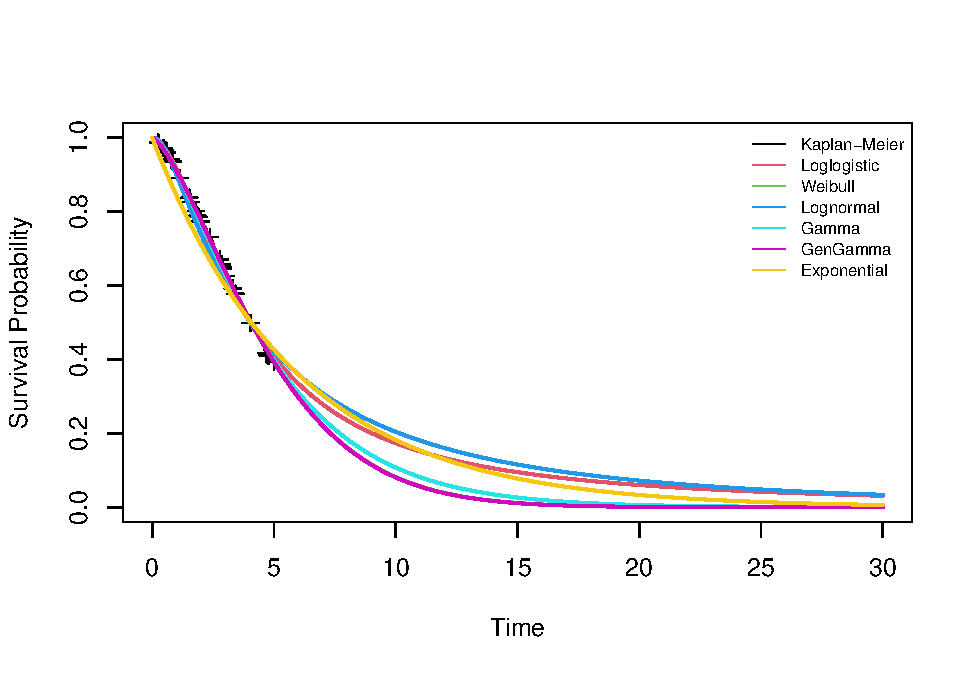
\includegraphics{CRS_Calib_NelderMead_files/figure-latex/unnamed-chunk-8-3.pdf}

\begin{Shaded}
\begin{Highlighting}[]
\CommentTok{# TARGET 2: (if you had more...)}
\CommentTok{# plotrix::plotCI(x = lst_targets$Target2$time, y = lst_targets$Target2$value, }
\CommentTok{#                 ui = lst_targets$Target2$ub,}
\CommentTok{#                 li = lst_targets$Target2$lb,}
\CommentTok{#                 ylim = c(0, 1), }
\CommentTok{#                 xlab = "Time", ylab = "Target 2")}
\CommentTok{# points(x = lst_targets$Target2$time, }
\CommentTok{#        y = v_out_best$Target2, }
\CommentTok{#        pch = 8, col = "red")}
\CommentTok{# legend("topright", }
\CommentTok{#        legend = c("Target", "Model-predicted output"),}
\CommentTok{#        col = c("black", "red"), pch = c(1, 8))}
\end{Highlighting}
\end{Shaded}

\end{document}
